% Options for packages loaded elsewhere
\PassOptionsToPackage{unicode}{hyperref}
\PassOptionsToPackage{hyphens}{url}
%
\documentclass[
]{article}
\usepackage{amsmath,amssymb}
\usepackage{lmodern}
\usepackage{ifxetex,ifluatex}
\ifnum 0\ifxetex 1\fi\ifluatex 1\fi=0 % if pdftex
  \usepackage[T1]{fontenc}
  \usepackage[utf8]{inputenc}
  \usepackage{textcomp} % provide euro and other symbols
\else % if luatex or xetex
  \usepackage{unicode-math}
  \defaultfontfeatures{Scale=MatchLowercase}
  \defaultfontfeatures[\rmfamily]{Ligatures=TeX,Scale=1}
\fi
% Use upquote if available, for straight quotes in verbatim environments
\IfFileExists{upquote.sty}{\usepackage{upquote}}{}
\IfFileExists{microtype.sty}{% use microtype if available
  \usepackage[]{microtype}
  \UseMicrotypeSet[protrusion]{basicmath} % disable protrusion for tt fonts
}{}
\makeatletter
\@ifundefined{KOMAClassName}{% if non-KOMA class
  \IfFileExists{parskip.sty}{%
    \usepackage{parskip}
  }{% else
    \setlength{\parindent}{0pt}
    \setlength{\parskip}{6pt plus 2pt minus 1pt}}
}{% if KOMA class
  \KOMAoptions{parskip=half}}
\makeatother
\usepackage{xcolor}
\IfFileExists{xurl.sty}{\usepackage{xurl}}{} % add URL line breaks if available
\IfFileExists{bookmark.sty}{\usepackage{bookmark}}{\usepackage{hyperref}}
\hypersetup{
  pdftitle={MATH 3080 Lab Project 3},
  pdfauthor={Harrison Webb},
  hidelinks,
  pdfcreator={LaTeX via pandoc}}
\urlstyle{same} % disable monospaced font for URLs
\usepackage[margin=1in]{geometry}
\usepackage{color}
\usepackage{fancyvrb}
\newcommand{\VerbBar}{|}
\newcommand{\VERB}{\Verb[commandchars=\\\{\}]}
\DefineVerbatimEnvironment{Highlighting}{Verbatim}{commandchars=\\\{\}}
% Add ',fontsize=\small' for more characters per line
\usepackage{framed}
\definecolor{shadecolor}{RGB}{248,248,248}
\newenvironment{Shaded}{\begin{snugshade}}{\end{snugshade}}
\newcommand{\AlertTok}[1]{\textcolor[rgb]{0.94,0.16,0.16}{#1}}
\newcommand{\AnnotationTok}[1]{\textcolor[rgb]{0.56,0.35,0.01}{\textbf{\textit{#1}}}}
\newcommand{\AttributeTok}[1]{\textcolor[rgb]{0.77,0.63,0.00}{#1}}
\newcommand{\BaseNTok}[1]{\textcolor[rgb]{0.00,0.00,0.81}{#1}}
\newcommand{\BuiltInTok}[1]{#1}
\newcommand{\CharTok}[1]{\textcolor[rgb]{0.31,0.60,0.02}{#1}}
\newcommand{\CommentTok}[1]{\textcolor[rgb]{0.56,0.35,0.01}{\textit{#1}}}
\newcommand{\CommentVarTok}[1]{\textcolor[rgb]{0.56,0.35,0.01}{\textbf{\textit{#1}}}}
\newcommand{\ConstantTok}[1]{\textcolor[rgb]{0.00,0.00,0.00}{#1}}
\newcommand{\ControlFlowTok}[1]{\textcolor[rgb]{0.13,0.29,0.53}{\textbf{#1}}}
\newcommand{\DataTypeTok}[1]{\textcolor[rgb]{0.13,0.29,0.53}{#1}}
\newcommand{\DecValTok}[1]{\textcolor[rgb]{0.00,0.00,0.81}{#1}}
\newcommand{\DocumentationTok}[1]{\textcolor[rgb]{0.56,0.35,0.01}{\textbf{\textit{#1}}}}
\newcommand{\ErrorTok}[1]{\textcolor[rgb]{0.64,0.00,0.00}{\textbf{#1}}}
\newcommand{\ExtensionTok}[1]{#1}
\newcommand{\FloatTok}[1]{\textcolor[rgb]{0.00,0.00,0.81}{#1}}
\newcommand{\FunctionTok}[1]{\textcolor[rgb]{0.00,0.00,0.00}{#1}}
\newcommand{\ImportTok}[1]{#1}
\newcommand{\InformationTok}[1]{\textcolor[rgb]{0.56,0.35,0.01}{\textbf{\textit{#1}}}}
\newcommand{\KeywordTok}[1]{\textcolor[rgb]{0.13,0.29,0.53}{\textbf{#1}}}
\newcommand{\NormalTok}[1]{#1}
\newcommand{\OperatorTok}[1]{\textcolor[rgb]{0.81,0.36,0.00}{\textbf{#1}}}
\newcommand{\OtherTok}[1]{\textcolor[rgb]{0.56,0.35,0.01}{#1}}
\newcommand{\PreprocessorTok}[1]{\textcolor[rgb]{0.56,0.35,0.01}{\textit{#1}}}
\newcommand{\RegionMarkerTok}[1]{#1}
\newcommand{\SpecialCharTok}[1]{\textcolor[rgb]{0.00,0.00,0.00}{#1}}
\newcommand{\SpecialStringTok}[1]{\textcolor[rgb]{0.31,0.60,0.02}{#1}}
\newcommand{\StringTok}[1]{\textcolor[rgb]{0.31,0.60,0.02}{#1}}
\newcommand{\VariableTok}[1]{\textcolor[rgb]{0.00,0.00,0.00}{#1}}
\newcommand{\VerbatimStringTok}[1]{\textcolor[rgb]{0.31,0.60,0.02}{#1}}
\newcommand{\WarningTok}[1]{\textcolor[rgb]{0.56,0.35,0.01}{\textbf{\textit{#1}}}}
\usepackage{longtable,booktabs,array}
\usepackage{calc} % for calculating minipage widths
% Correct order of tables after \paragraph or \subparagraph
\usepackage{etoolbox}
\makeatletter
\patchcmd\longtable{\par}{\if@noskipsec\mbox{}\fi\par}{}{}
\makeatother
% Allow footnotes in longtable head/foot
\IfFileExists{footnotehyper.sty}{\usepackage{footnotehyper}}{\usepackage{footnote}}
\makesavenoteenv{longtable}
\usepackage{graphicx}
\makeatletter
\def\maxwidth{\ifdim\Gin@nat@width>\linewidth\linewidth\else\Gin@nat@width\fi}
\def\maxheight{\ifdim\Gin@nat@height>\textheight\textheight\else\Gin@nat@height\fi}
\makeatother
% Scale images if necessary, so that they will not overflow the page
% margins by default, and it is still possible to overwrite the defaults
% using explicit options in \includegraphics[width, height, ...]{}
\setkeys{Gin}{width=\maxwidth,height=\maxheight,keepaspectratio}
% Set default figure placement to htbp
\makeatletter
\def\fps@figure{htbp}
\makeatother
\setlength{\emergencystretch}{3em} % prevent overfull lines
\providecommand{\tightlist}{%
  \setlength{\itemsep}{0pt}\setlength{\parskip}{0pt}}
\setcounter{secnumdepth}{-\maxdimen} % remove section numbering
\ifluatex
  \usepackage{selnolig}  % disable illegal ligatures
\fi

\title{MATH 3080 Lab Project 3}
\author{Harrison Webb}
\date{12/29/2019}

\begin{document}
\maketitle

{
\setcounter{tocdepth}{2}
\tableofcontents
}
\hypertarget{problem-1-verzani-problem-12.2}{%
\section{Problem 1 (Verzani problem
12.2)}\label{problem-1-verzani-problem-12.2}}

\emph{For the data set \texttt{Cars93} (\textbf{MASS}) perform a one-way
analysis of variance of \texttt{MPG.highway} for each level of
\texttt{DriveTrain}. Does the data support the null hypothesis of equal
population means? (Use \texttt{aov()} for this problem.)}

\begin{Shaded}
\begin{Highlighting}[]
\CommentTok{\#check equal variances}
\FunctionTok{boxplot}\NormalTok{(MPG.highway}\SpecialCharTok{\textasciitilde{}}\NormalTok{DriveTrain, }\AttributeTok{data =}\NormalTok{ Cars93)}
\end{Highlighting}
\end{Shaded}

\begin{figure}
\centering
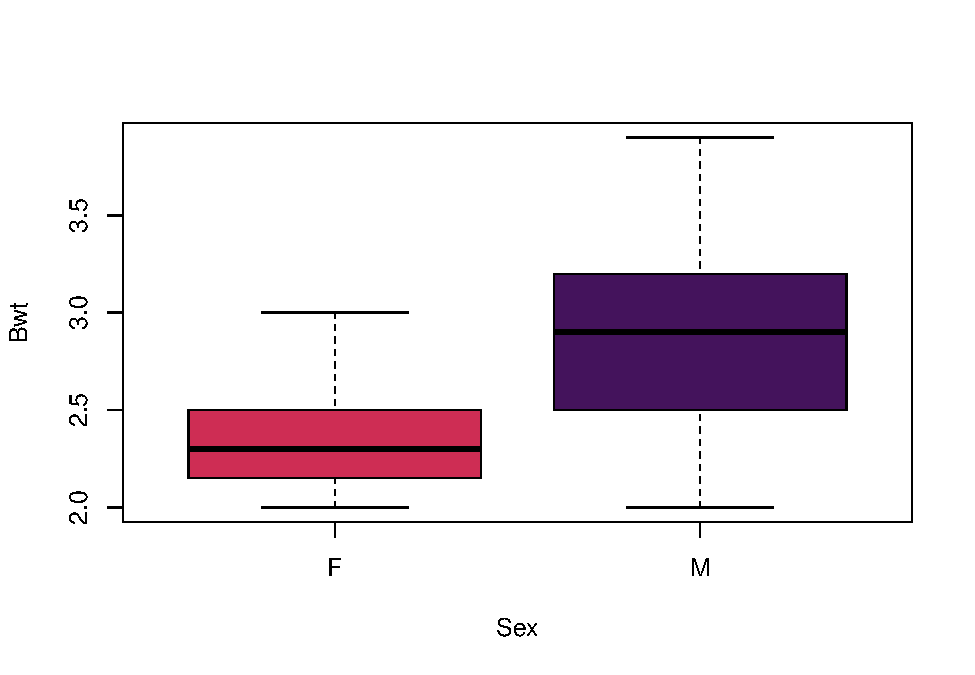
\includegraphics{3080Project3_ANOVA_files/figure-latex/unnamed-chunk-2-1.pdf}
\caption{Variances appear to differ a bit more than we would like, but
we will still carryout the test}
\end{figure}

\begin{Shaded}
\begin{Highlighting}[]
\CommentTok{\#check normality}
\FunctionTok{shapiro.test}\NormalTok{(Cars93}\SpecialCharTok{$}\NormalTok{MPG.highway)}
\end{Highlighting}
\end{Shaded}

\begin{verbatim}
## 
##  Shapiro-Wilk normality test
## 
## data:  Cars93$MPG.highway
## W = 0.92443, p-value = 4.576e-05
\end{verbatim}

\begin{Shaded}
\begin{Highlighting}[]
\CommentTok{\#conduct ANOVA test}
\NormalTok{result }\OtherTok{=} \FunctionTok{aov}\NormalTok{(MPG.highway}\SpecialCharTok{\textasciitilde{}}\NormalTok{DriveTrain, }\AttributeTok{data =}\NormalTok{ Cars93)}
\FunctionTok{summary}\NormalTok{(result)}
\end{Highlighting}
\end{Shaded}

\begin{verbatim}
##             Df Sum Sq Mean Sq F value  Pr(>F)   
## DriveTrain   2  320.1   160.1   6.276 0.00281 **
## Residuals   90 2295.2    25.5                   
## ---
## Signif. codes:  0 '***' 0.001 '**' 0.01 '*' 0.05 '.' 0.1 ' ' 1
\end{verbatim}

\hypertarget{problem-2-verzani-problem-12.4}{%
\section{Problem 2 (Verzani problem
12.4)}\label{problem-2-verzani-problem-12.4}}

\emph{The data set \texttt{carsafety} (\textbf{UsingR}) contains
car-crash data. For several makes of cars the number of drivers killed
per million is recorded in \texttt{Drivers.deaths}. The number of
drivers of other cars killed in accidents with these cars, per million,
is recorded in \texttt{Other.deaths}. The variable \texttt{type} is a
factor indicating the type of car.}

\emph{Perform a one-way analysis of variance of the model
\texttt{Drivers.deaths\ \textasciitilde{}\ type}. Is there a difference
in population means? Did you assume equal variances? Normally
distributed populations?}

\emph{Repeat with an analysis of variance of the model
\texttt{Other.deaths\ \textasciitilde{}\ type}. Is there a difference in
population means? (Use \texttt{oneway.test()} for this problem.)}

\begin{Shaded}
\begin{Highlighting}[]
\CommentTok{\# Your code here}
\end{Highlighting}
\end{Shaded}

\hypertarget{problem-3-verzani-problem-12.7}{%
\section{Problem 3 (Verzani problem
12.7)}\label{problem-3-verzani-problem-12.7}}

\emph{A manufacturer of point-of-sale merchandise tests three types of
ENTER-button markings. They wish to minimize wear, as customers get
annoyed when the markings on this button wear off. They construct a test
of the three types, and conduct several trials for each. The results, in
unspecified units, are recorded in the following table:}

\begin{longtable}[]{@{}lllllll@{}}
\toprule
& & & & & & \\
\midrule
\endhead
Type 1 & 303 & 293 & 296 & 299 & 298 & \\
Type 2 & 322 & 326 & 315 & 318 & 320 & 320 \\
Type 3 & 309 & 327 & 317 & 315 & & \\
\bottomrule
\end{longtable}

\emph{Is there a difference in wear time among the three types? Answer
this using a one-way ANOVA.}

\begin{Shaded}
\begin{Highlighting}[]
\CommentTok{\# Your code here}
\CommentTok{\#make one vector for types and another for \#s}
\end{Highlighting}
\end{Shaded}

\hypertarget{problem-4-verzani-problem-12.13}{%
\section{Problem 4 (Verzani problem
12.13)}\label{problem-4-verzani-problem-12.13}}

\emph{For the data in Problem 2, perform the one-way ANOVA using
\texttt{lm()}. Compare to the results of \texttt{oneway.test()}.}

\begin{Shaded}
\begin{Highlighting}[]
\CommentTok{\# Your code here}
\end{Highlighting}
\end{Shaded}

\hypertarget{problem-5-verzani-problem-12.19}{%
\section{Problem 5 (Verzani problem
12.19)}\label{problem-5-verzani-problem-12.19}}

\emph{The \texttt{InsectSprays} data set contains a variable
\texttt{count}, which counts the number of insects and a factor
\texttt{spray}, which indicates the treatment given.}

\emph{First perform an analysis of variance to see whether the
treatments make a difference. If so, perform the Tukey HSD procedure to
see which pairwise treatments differ.}

\begin{Shaded}
\begin{Highlighting}[]
\CommentTok{\# Your code here}
\end{Highlighting}
\end{Shaded}


\end{document}
